\documentclass[12pt,letterpaper,twoside]{article}
\usepackage{cme211}
\usepackage{algorithm2e}

\def\D{\mathrm{d}}
\usepackage{atbegshi}% http://ctan.org/pkg/atbegshi
\AtBeginDocument{\AtBeginShipoutNext{\AtBeginShipoutDiscard}}

\begin{document}
\title{Lecture 15: Boost\vspace{-5ex}}
\date{November 15th, 2018}
\maketitle

{\footnotesize
\paragraph{Topics:} Boost Library and multi-dimensional data.
}
\vspace{-3ex}

\section{Layout in Memory for a \texttt{std::vector}}

\begin{figure}[h]
\centering
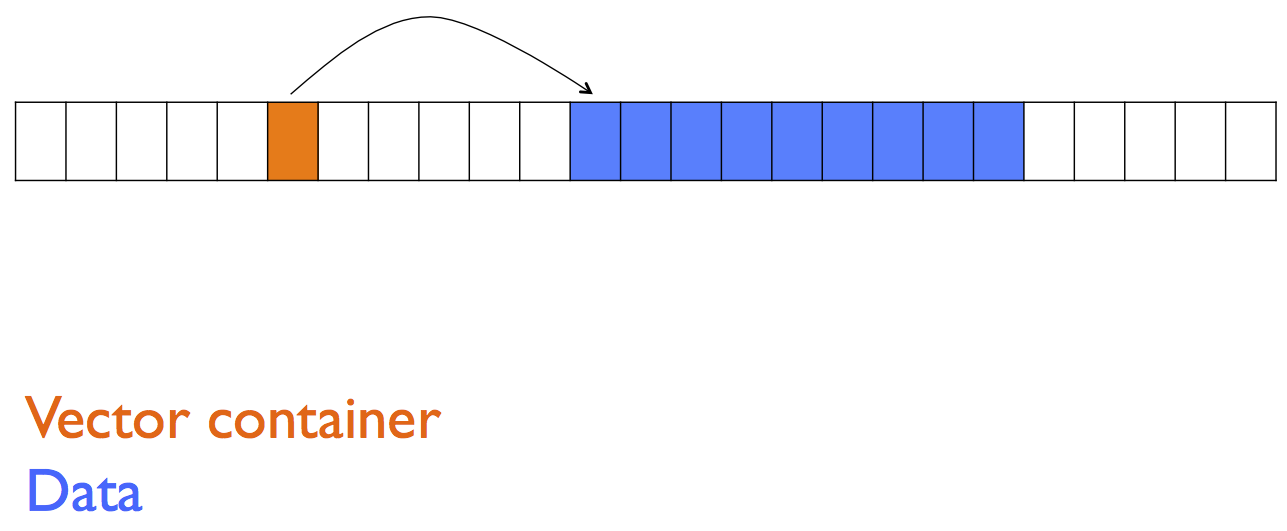
\includegraphics[scale=0.5]{fig/vector-memory.png}
\caption{\footnotesize 
  Suppose we initialize a vector, e.g. \texttt{std::vector<int> a = \{42, 0, 7\};}.
  There are a few data attributes that the \texttt{vector} class stores, such as 
  \texttt{size} and \texttt{capacity} of the vector as well as where the underlying data are stored
  in memory. Attributes such as \texttt{unsigned size}, \texttt{unsigned capacity}, and even the 
  memory address (describing where the \texttt{data} live in heap-allocated memory) 
  all reside within the orange cell of memory in the above diagram. When we inspect the value 
  of the \texttt{data} pointer and inspect the data that live at this location, we will find a bit 
  representation describing the integer values stored in our array.}
\end{figure}

Memory for \texttt{std::vector} has 2 parts, which may be very far apart in memory address space:
\begin{itemize}
\item
  Memory for the \texttt{std::vector} container. This part
  includes data attributes describing the memory address of the vector data, the
  size of the vector, and its allocation capacity.
\item
  An entirely separate section of memory for the contiguously allocated vector data.
\end{itemize}

The size of the \texttt{std::vector} container is 24 bytes, this \emph{could}
be for:
\begin{itemize}
  \item 8 bytes for the memory address of the vector \texttt{data},
  \item 8 bytes for the \texttt{size} of the vector, number of elements \emph{currently stored}, and
  \item 8 bytes of the \texttt{capacity} of the vector, number of elements that 
    \emph{may be stored} before reallocation is required.
\end{itemize}
Memory locations are different in each run of the program. This is a
security feature to make it harder to introduce malicious code or
data.

\paragraph{Look at the Details} Consider an example from
\texttt{src/vector\_memory.cpp}:

\begin{cpp}
#include <iostream>
#include <vector>
 int main() {
  std::vector<int> a;
  for (int i = 0; i < 10; i++)
      a.push_back(i);
  std::cout << "sizeof(a)  : " << sizeof(a)   << std::endl;
  std::cout << "sizeof(int): " << sizeof(int) << std::endl;
  std::cout << "memory location of    a : " << &a << std::endl;
  std::cout << "memory location of data : " << a.data() << std::endl;
  std::cout << "memory location of a[0] : " << &a[0] << std::endl;  // Postfix operators bind tighter.
  std::cout << "memory location of a[1] : " << &a[1] << std::endl;
  return 0;
}
\end{cpp}

Output after compiling with \texttt{g++ -std=c++11 vector\_memory.cpp -o vector\_memory}:

{
\footnotesize
\begin{verbatim}
./vector_memory
sizeof(a)  : 24
sizeof(int): 4
memory location of    a : 0x7ffcdc97df40
memory location of data : 0x6a8c90
memory location of a[0] : 0x6a8c90
memory location of a[1] : 0x6a8c94
./vector_memory
sizeof(a)  : 24
sizeof(int): 4
memory location of    a : 0x7ffdbeac7b70
memory location of data : 0x1600c90
memory location of a[0] : 0x1600c90
memory location of a[1] : 0x1600c94
\end{verbatim}
}

Note that at an even lower level of abstraction, and beyond our control as C++ programmers, 
the operating system may use 
\href{https://en.wikipedia.org/wiki/Virtual_memory}{\emph{virtual memory}}, which in this example
could make the difference in memory location between \texttt{a} and \texttt{a.data()} to 
\emph{appear} larger than available RAM.

\vspace{-2ex}
\subsection{Multidimensional Data via Nested \texttt{std::vector}s}
\label{sec: nested-vectors}
One approach to multidimensional data in C++ is using nested containers, e.g.
\texttt{src/multi1.cpp}:

\begin{cpp}
#include <vector>
#include <iostream>
 int main() {
  std::vector< std::vector<double>> v;                     // Declare a vector of vectors.
  for (int i = 0; i < 3; i++) 
    v.push_back(std::vector<double>());
  int n = 0;                                               // Add some data
  for(unsigned int i = 0; i < 3; i++)
    for(unsigned int j = 0; j < 3; j++)
      v[i].push_back(n++);
  std::cout << "sizeof(v): " << sizeof(v) << std::endl;    // Print vector information...
  for(unsigned int i = 0; i < 3; i++)
    for(unsigned int j = 0; j < 3; j++)
      std::cout << "v[" << i << "][" << j << "] = " << v[i][j] << std::endl;
}
\end{cpp}

Output after compiling
{\small \texttt{g++ -std=c++11 src/multi1.cpp -o src/multi1}}:

{\small
\begin{verbatim}
$ ./src/multi1
v[0][0] = 0
v[0][1] = 1
v[0][2] = 2
v[1][0] = 3
v[1][1] = 4
v[1][2] = 5
v[2][0] = 6
v[2][1] = 7
v[2][2] = 8
\end{verbatim}
}

What's the \emph{layout in memory}?
\begin{figure}[h]
\centering
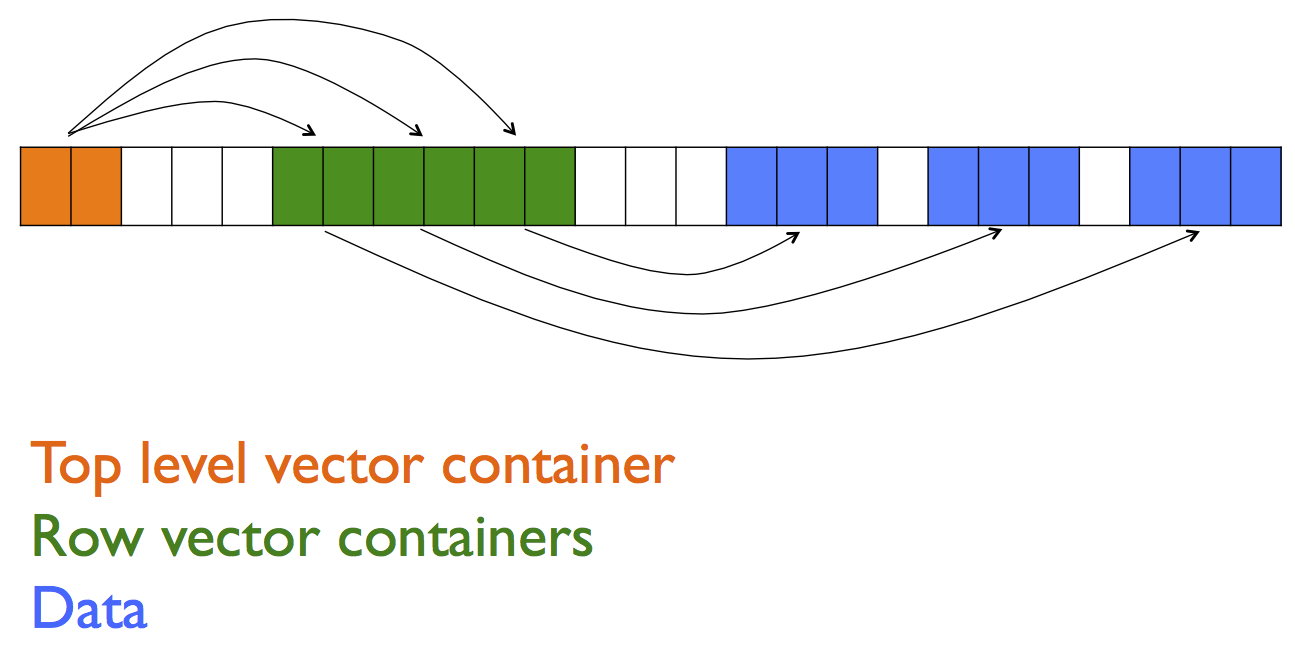
\includegraphics[scale=0.5]{fig/vector-of-vectors.png}
\caption{\footnotesize 
  In this figure, we use ``two orange blocks'' to refer to the top level container, but note
  that \texttt{sizeof(std::vector<std::vector>>)} is the same as \texttt{sizeof(std::vector<int>)}, 
  since the top level container only stores a pointer to \texttt{data}, \texttt{size}, and 
  \texttt{capacity}. When we examine the \texttt{data} pointer for the top level container, 
  it refers 
  to a sequence of bits in memory describing each \emph{row} vector container (green). 
  These row vectors in 
  turn have \texttt{data} pointers which refer to elements contiguously allocated in memory (blue).}
\label{fig: nested-vectors}
\end{figure}

The above approach may not be ideal depending on the application or context of use. For example,
if we use nested containers (as above) to implement a numeric \texttt{matrix} data-structure, then
if we try to perform operations ``by column'' we will suffer from 
\href{https://en.wikipedia.org/wiki/CPU_cache#Cache_miss}{cache-misses}: i.e. the elements
within a single column lay very far apart from each other in memory in figure 
\ref{fig: nested-vectors}.

\subsection{Multidimensional Data via ``Flat'' \texttt{std::vector} and Offsets} 
\label{sec: multid-arr-via-offsets}
We can instead use a \texttt{std::vector>} (\emph{not} nested)
where we manually apply an offset to translate a tuple into an index. I.e. if we wish to represent
an $n \times p$ matrix in 
\href{https://en.wikipedia.org/wiki/Row-_and_column-major_order}{\emph{row-major} order}, 
then (assuming 0-based indexing) $(i,j) \leadsto i*p + j$; see
\texttt{src/multi2.cpp}:

\begin{cpp}
#include <iostream>
#include <vector>

int main() {
  unsigned int nrows = 3, ncols = 3;
  std::vector<double> a;
  a.resize(nrows*ncols);

  double n = 0.;
  for(unsigned int i = 0; i < nrows; i++)
    for(unsigned int j = 0; j < ncols; j++)
      a[i*ncols + j] = n++; // manual indexing into "multi-dimensional array".

  for(unsigned int i = 0; i < nrows*ncols; i++)
    std::cout << "a[" << i << "] = " << a[i] << std::endl;
}
\end{cpp}

Output after \texttt{g++ -std=c++11 src/multi2.cpp -o src/multi2}:

{\small
\begin{verbatim}
$ ./src/multi2
a[0] = 0
a[1] = 1
a[2] = 2
a[3] = 3
a[4] = 4
a[5] = 5
a[6] = 6
a[7] = 7
a[8] = 8
\end{verbatim}
}

\section{Boost Multidimensional Array Library}
Let's turn to a library totally separate from the 
\href{https://en.wikipedia.org/wiki/Standard_Template_Library}{C++ standard template library}.
Boost is a very large library, and one piece of functionality it affords us is a 
\emph{multi-dimensional} array in which the data are contiguously allocated in memory. Relative
to what we described above, it combines a ``best of both worlds'': we may index into 
an \texttt{n}-dimensional array using \emph{n-levels} of indirection \texttt{[]} 
(similar to our approach in section \ref{sec: nested-vectors}) but the underlying
data are laid out contiguously (similar to our approach in section 
\ref{sec: multid-arr-via-offsets}); see
\texttt{src/array1.cpp}:

\begin{cpp}
#include <iostream>
#include <boost/multi_array.hpp>

int main() {
  unsigned int nrows = 3, ncols = 3;
  boost::multi_array<double, 2> a(boost::extents[nrows][ncols]);
  int n = 0;
  for (unsigned int i = 0; i < nrows; i++)
    for (unsigned int j = 0; j < ncols; j++)
      a[i][j] = n++; // access elements like static array

  for (unsigned int i = 0; i < nrows; i++)
    for (unsigned int j = 0; j < ncols; j++)
      std::cout << "a[" << i << "][" << j << "] = " << a[i][j] << std::endl;
}
\end{cpp}

Output:

\begin{verbatim}
$ g++ -std=c++11 -Wall -Wextra -Wconversion src/array1.cpp -o src/array1
$ ./src/array1
a[0][0] = 0
a[0][1] = 1
a[0][2] = 2
a[1][0] = 3
a[1][1] = 4
a[1][2] = 5
a[2][0] = 6
a[2][1] = 7
a[2][2] = 8
\end{verbatim}

\subsection{Demonstration: Elements Contiguously Allocated in Memory} How can we be sure
our data elements are contiguously allocated? We can use pointer-arithmetic; see
\texttt{src/array2.cpp}:

\begin{cpp}
#include <iostream>
#include <boost/multi_array.hpp>

int main() {
  boost::multi_array<double, 2> a(boost::extents[3][3]);
  int n = 0;
  for (unsigned int i = 0; i < 3; i++)
    for (unsigned int j = 0; j < 3; j++)
      a[i][j] = n++;

  for (unsigned int n = 0; n < a.num_elements(); n++)
    std::cout << "a.data()[" << n << "] = " << a.data()[n] << std::endl;
}
\end{cpp}

Note that we are populating our array using 2 levels of indirection via \texttt{[][]}, but when we
print our elements we are only using a single level of indirection.

\begin{verbatim}
$ g++ -std=c++11 -Wall -Wextra -Wconversion src/array2.cpp -o src/array2
$ ./src/array2
a.data()[0] = 0
a.data()[1] = 1
a.data()[2] = 2
a.data()[3] = 3
a.data()[4] = 4
a.data()[5] = 5
a.data()[6] = 6
a.data()[7] = 7
a.data()[8] = 8
\end{verbatim}

\subsection{Performance of Boost vs. Static Arrays}
Suppose we try and sum all the elements in a 2D array. How does Boost compare with static arrays?
See \texttt{src/perf1.cpp}:

\begin{cpp}
#include <iostream>
#include <ctime>
#include <boost/multi_array.hpp>

int main() {
  unsigned int nrows = 8192, ncols = 8192;
  boost::multi_array<int, 2> a(boost::extents[nrows][ncols]);

  // Initialize boost array with 2^13 x 2^13 elements, each with unit value.
  for (unsigned int i = 0; i < nrows; i++)
    for (unsigned int j = 0; j < ncols; j++)
      a[i][j] = 1;
  // How fast can we sum the elements?
  auto t0 = std::clock();
  int sum = 0;
  for (unsigned int i = 0; i < nrows; i++)
    for (unsigned int j = 0; j < ncols; j++)
      sum += a[i][j];
  auto t1 = std::clock();
  std::cout << " boost: sum = " << sum << ", time = "
            << double(t1-t0) / CLOCKS_PER_SEC
            << " seconds"<< std::endl;

  // Repeat, this time using a flat-array! (Recall, a.data() is an int*)
  auto b = a.data();
  t0 = std::clock();
  sum = 0;
  for (unsigned int n = 0; n < nrows*ncols; n++)
    sum += b[n];
  t1 = std::clock();

  std::cout << "direct: sum = " << sum << ", time = "
            << double(t1-t0) / CLOCKS_PER_SEC
            << " seconds"<< std::endl;
}
\end{cpp}

We might at first be disappointed in the output:

{\small
\begin{verbatim}
$ clang++ -std=c++11 -Wall -Wextra -Wconversion src/perf1.cpp -o src/perf1
$ ./src/perf1
 boost: sum = 6.71089e+07, time = 4.55984 seconds
direct: sum = 6.71089e+07, time = 0.240126 seconds
$ ./src/perf1
 boost: sum = 6.71089e+07, time = 4.41117 seconds
direct: sum = 6.71089e+07, time = 0.228782 seconds
$ ./src/perf1
 boost: sum = 6.71089e+07, time = 4.38506 seconds
direct: sum = 6.71089e+07, time = 0.235112 seconds
\end{verbatim}
}

\subsubsection{Disabling Range-Checking in Boost}
Note that by default, Boost enables range-checking, and this incurs some cost;
\texttt{src/perf2.cpp}:

\begin{cpp}
// disable boost range checking
#define BOOST_DISABLE_ASSERTS
#include <boost/multi_array.hpp>
\end{cpp}

With the rest of the program unchanged, we see a small performance increase:
{\small
\begin{verbatim}
$ clang++ -std=c++11 -Wall -Wextra -Wconversion src/perf2.cpp -o src/perf2
$ ./src/perf2
 boost: sum = 6.71089e+07, time = 4.4622 seconds
direct: sum = 6.71089e+07, time = 0.235016 seconds
$ ./src/perf2
 boost: sum = 6.71089e+07, time = 4.26261 seconds
direct: sum = 6.71089e+07, time = 0.226978 seconds
$ ./src/perf2
 boost: sum = 6.71089e+07, time = 4.2159 seconds
direct: sum = 6.71089e+07, time = 0.240271 seconds
\end{verbatim}
}

\subsubsection{Compiler Optimizations}
Let's enable compiler optimizations with the \texttt{-O3} argument.\footnote{It's harder for 
the compiler to reason about a boost multi-dimensional array than it is to reason about a built-in
static array. Therefore, unless we ask the compiler to be aggressive with optimizations, it may
miss out on applying optimizations it would have otherwise to the static arrays. Some of these
optimizations could include, for example 
\href{https://en.wikipedia.org/wiki/Loop_unrolling}{loop-unrolling}.}
With range checking:

{\small
\begin{verbatim}
$ g++ -O3 -std=c++11 -Wall -Wextra -Wconversion src/perf1.cpp -o src/perf1
$ ./src/perf1
 boost: sum = 6.71089e+07, time = 0.102904 seconds
direct: sum = 6.71089e+07, time = 0.107179 seconds
$ ./src/perf1
 boost: sum = 6.71089e+07, time = 0.119958 seconds
direct: sum = 6.71089e+07, time = 0.121643 seconds
$ ./src/perf1
 boost: sum = 6.71089e+07, time = 0.10259 seconds
direct: sum = 6.71089e+07, time = 0.105372 seconds
\end{verbatim}
}

\emph{Without range} checking:
{\small
\begin{verbatim}
$ g++ -O3 -std=c++11 -Wall -Wextra -Wconversion src/perf2.cpp -o src/perf2
$ ./src/perf2
 boost: sum = 6.71089e+07, time = 0.102209 seconds
direct: sum = 6.71089e+07, time = 0.102016 seconds
$ ./src/perf2
 boost: sum = 6.71089e+07, time = 0.104234 seconds
direct: sum = 6.71089e+07, time = 0.105256 seconds
$ ./src/perf2
 boost: sum = 6.71089e+07, time = 0.101876 seconds
direct: sum = 6.71089e+07, time = 0.117592 seconds
\end{verbatim}
}

\subsection{Range Checking} Let's consider the behavior of range-checking in Boost; by default
it's similar to using the \texttt{at()} method for a \texttt{vector}. See
\texttt{src/array3a.cpp}:

\begin{cpp}
#include <iostream>
#include <boost/multi_array.hpp>

int main() {
  boost::multi_array<double, 2> a(boost::extents[3][3]);
  a[3][3] = 1.;
}
\end{cpp}

{\small
\begin{verbatim}
$ g++ -std=c++11 -Wall -Wextra -Wconversion src/array3a.cpp -o src/array3a
$ ./src/array3a
Assertion failed: (size_type(idx - index_bases[0]) < extents[0]), function
access, file /usr/local/include/boost/multi_array/base.hpp, line 136.
\end{verbatim}
}

We can \emph{manually disable boost asserts}, in which case
the code compiles without warning.
\begin{cpp}
#include <iostream>
#define BOOST_DISABLE_ASSERTS
#include <boost/multi_array.hpp>
int main() {
  boost::multi_array<double, 2> a(boost::extents[3][3]);
  a[3][3] = 1.;
}
\end{cpp}

{\small
\begin{verbatim}
$ g++ -std=c++11 -Wall -Wextra -Wconversion src/array3b.cpp -o src/array3b
$ ./src/array3b
\end{verbatim}
}

\subsubsection{Range Checking Via Address Sanitizer}
However, if we were to enable 
\href{https://en.wikipedia.org/wiki/AddressSanitizer}{address sanitizer}, 
we would be alerted to an invalid write.

{\small
\begin{verbatim}
$ g++ -std=c++11 -g -fsanitize=address -Wall -Wextra -Wconversion src/array3b.cpp \
  -o src/array3b
$ ./src/array3b
==36808==ERROR: AddressSanitizer: heap-buffer-overflow on address 0x60700000df30 ...
WRITE of size 8 at 0x60700000df30 thread T0
    #0 0x10dc1aad4 in main array3b.cpp:7
    #1 0x7fff9426d5ac in start (libdyld.dylib+0x35ac) ...
0x60700000df30 is located 16 bytes to the left of 67-byte region
... (Output omitted)
SUMMARY: AddressSanitizer: heap-buffer-overflow array3b.cpp:7 in main
Shadow bytes around the buggy address:
  0x1c0e00001bd0: fa fa fa fa fa fa fa fa fa fa 00 00 00 00 00 00
=>0x1c0e00001be0: 00 00 00 fa fa fa[fa]fa 00 00 00 00 00 00 00 00
  0x1c0e00001bf0: 03 fa fa fa fa fa 00 00 00 00 00 00 00 00 00 fa
... (Output omitted)
==36808==ABORTING
\end{verbatim}
}

\subsubsection{Range Checking via Valgrind}
Another method to check for memory leaks is 
\href{https://en.wikipedia.org/wiki/Valgrind}{\texttt{valgrind}}.
For the same program, enabling the \texttt{-g} debug mode and running under \texttt{valgrind}:

{\footnotesize
\begin{verbatim}
$ g++ -g -Wall -Wextra -Wconversion src/array3b.cpp -o src/array3b
$ valgrind ./src/array3b
==36817== Memcheck, a memory error detector
==36817== Copyright (C) 2002-2015, and GNU GPL'd, by Julian Seward et al.
==36817== Using Valgrind-3.12.0 and LibVEX; rerun with -h for copyright info
==36817== Command: ./src/array3b
==36817== 
==36817== Invalid write of size 8
==36817==    at 0x10000109D: main (array3b.cpp:7)
==36817==  Address 0x100a88180 is 16 bytes after a block of size 80 in arena "client"
==36817== 
==36817== HEAP SUMMARY:
==36817==     in use at exit: 22,458 bytes in 194 blocks
==36817==   total heap usage: 258 allocs, 64 frees, 28,226 bytes allocated
==36817== 
==36817== LEAK SUMMARY:
==36817==    definitely lost: 0 bytes in 0 blocks
==36817==    indirectly lost: 0 bytes in 0 blocks
==36817==      possibly lost: 2,064 bytes in 1 blocks
==36817==    still reachable: 0 bytes in 0 blocks
==36817==         suppressed: 20,394 bytes in 193 blocks
==36817== Rerun with --leak-check=full to see details of leaked memory
==36817== 
==36817== For counts of detected and suppressed errors, rerun with: -v
==36817== ERROR SUMMARY: 1 errors from 1 contexts (suppressed: 0 from 0)
\end{verbatim}
}

\subsection{Overloaded Operators: Comparison and Assignment}
\subsubsection{Elementwise Comparison} The comparison operators have been overloaded by 
Boost authors to perform elementwise comparison across compatibly sized multi-arrays and return
a single Boolean;
\texttt{src/array5.cpp}:

\begin{cpp}
#include <iostream>
#include <boost/multi_array.hpp>
int main() {
  boost::multi_array<double, 2> a(boost::extents[3][3]);
  boost::multi_array<double, 2> b(boost::extents[3][3]);
  for (unsigned int i = 0; i < 3; i++) {
    for (unsigned int j = 0; j < 3; j++) {
      a[i][j] = 1.;
      b[i][j] = 2.;
    }
  }
  std::cout << "a == b: " << (a == b) << std::endl;
  std::cout << "a  < b: " << (a  < b) << std::endl;
  std::cout << "a  > b: " << (a  > b) << std::endl;
}
\end{cpp}

Output:

\begin{verbatim}
$ g++ -std=c++11 -Wall -Wextra -Wconversion src/array5.cpp -o src/array5
$ ./src/array5
a == b: 0
a  < b: 1
a  > b: 0
\end{verbatim}

\subsubsection{Assignment Operator Copies Underlying Elements} 
When the authors of Boost chose to overload \texttt{operator=} such that it can apply
to a multi-array, they had to decide whether to create a copy of the underlying elements;
\texttt{src/array6a.cpp}:

\begin{cpp}
#include <iostream>
#include <boost/multi_array.hpp>

int main() {
  boost::multi_array<double, 2> a(boost::extents[3][3]);
  for (unsigned int i = 0; i < 3; i++) {
    for (unsigned int j = 0; j < 3; j++) {
      a[i][j] = 1.;
    }
  }

  auto b = a; // copy or reference? Authors chose to overload operator= to copy.
  for (unsigned int i = 0; i < 3; i++)
    for (unsigned int j = 0; j < 3; j++)
      a[i][j] = 2.;

  std::cout << "a b" << std::endl;
  std::cout << "---" << std::endl;
  for (unsigned int i = 0; i < 3; i++)
    for (unsigned int j = 0; j < 3; j++)
      std::cout << a[i][j] << " " << b[i][j] << std::endl;
}
\end{cpp}

Output:

\begin{verbatim}
$ clang++ -std=c++11 -Wall -Wextra -Wconversion src/array6a.cpp -o src/array6a
$ ./src/array6a
a b
---
2 1
2 1
2 1
2 1
2 1
2 1
2 1
2 1
2 1
\end{verbatim}

\subsection{Passing a Multi-Array to a Function}
\subsubsection{Default is for Multi-Arrays to be Passed-by-Value}
Similarly, Boost multi-arrays are
passed \emph{by value} into other functions, i.e. our underlying data are copied and we 
\emph{do not} have a reference to the original data we passed in; 
\texttt{src/array6b.cpp}:

\begin{cpp}
#include <iostream>
#include <boost/multi_array.hpp>

void increment(boost::multi_array<double, 2> b) {
  for (unsigned int i = 0; i < 3; i++)
    for (unsigned int j = 0; j < 3; j++)
      b[i][j]++;
}

int main() {
  boost::multi_array<double, 2> a(boost::extents[3][3]);

  // Initialize elements of 'a' to unit value.
  for (unsigned int i = 0; i < 3; i++)
    for (unsigned int j = 0; j < 3; j++)
      a[i][j] = 1.;
      
  // Niavely request elements of 'a' be incremented...
  increment(a);    // ... but variable 'a' is passed by value! Whence 'a' is _not_ incremented.

  // Observe the contents of 'a' still contain unit value.
  for (unsigned int i = 0; i < 3; i++)
    for (unsigned int j = 0; j < 3; j++)
      std::cout << a[i][j] << std::endl;
}
\end{cpp}

When we pass \texttt{a} to \texttt{increment}, we created a \emph{new} 
\texttt{boost::multi\_array<double, 2>} and specified that each element shall be initialized
with a copy of the underlying element in the multi-array \texttt{a} which was passed.

\begin{verbatim}
$ g++ -std=c++11 -Wall -Wextra -Wconversion src/array6b.cpp -o src/array6b
$ ./src/array6b
1
1
1
1
1
1
1
1
1
\end{verbatim}

\subsubsection{Passing by Reference}
We can specify that we desire an argument to be passed by reference by specifying the argument type
itself to be a reference, using the character \texttt{\&};
from \texttt{src/array6c.cpp}:

\begin{cpp}
void increment(boost::multi_array<double, 2>& b) {
  for (unsigned int i = 0; i < 3; i++) {
    for (unsigned int j = 0; j < 3; j++) {
      b[i][j]++;
    }
  }
}
\end{cpp}

In CME 212, we'll emphasize the relationship between pointers and references: references cannot be 
\texttt{NULL} and they can only be used to refer to a single object.
Output:

\begin{verbatim}
$ g++ -std=c++11 -Wall -Wextra -Wconversion src/array6c.cpp -o src/array6c
$ ./src/array6c
2
2
2
2
2
2
2
2
2
\end{verbatim}

\subsection{Other Array Operations?}
Boost \texttt{multi\_array} does not support array operations like
\texttt{NumPy}.
If \texttt{a} is a \texttt{multi\_array} things like \texttt{2*a} and
\texttt{a\ =\ 1.0} will not work and will lead to very long compiler
error messages.
If you want this kind of stuff, have a look at:

\begin{itemize}
\item
  \url{http://eigen.tuxfamily.org/index.php?title=Main\_Page}
\item
  \url{http://arma.sourceforge.net/}
\item
  \url{https://github.com/arrayfire/arrayfire}
\end{itemize}

\subsection{Array Views}
An \textbf{array view} is essentially a reference into a sub-array of a
larger array;
\texttt{src/array9.cpp}:

\begin{cpp}
#include <iostream>
#include <boost/multi_array.hpp>

int main() {
  boost::multi_array<double, 2> a(boost::extents[3][3]);

  double n = 0.;
  for (unsigned int i = 0; i < 3; i++)
    for (unsigned int j = 0; j < 3; j++)
      a[i][j] = n++;

  /* Setup b as a view into a subset of a. */
  typedef boost::multi_array<double, 2>::index_range index_range;
  auto b = a[boost::indices[index_range(1,3)][index_range(1,3)]];

  for (unsigned int i = 0; i < 2; i++)
    for (unsigned int j = 0; j < 2; j++)
      b[i][j] = -1.;

  for (unsigned int i = 0; i < 3; i++)
    for (unsigned int j = 0; j < 3; j++)
      std::cout << a[i][j] << std::endl;
}
\end{cpp}

Output:

\begin{verbatim}
$ clang++ -std=c++11 -Wall -Wextra -Wconversion src/array9.cpp -o src/array9
$ ./src/array9
0
1
2
3
-1
-1
6
-1
-1
\end{verbatim}

\subsection{Storage Order}
Boost uses the C convention that rows are stored contiguously in memory (row
major order); see
\texttt{src/array10a.cpp}:

\begin{cpp}
#include <iostream>
#include <boost/multi_array.hpp>

int main() {
  boost::multi_array<double, 2> a(boost::extents[3][3]);

  double n = 0.;
  for (unsigned int i = 0; i < 3; i++)
    for (unsigned int j = 0; j < 3; j++)
      a[i][j] = n++;

  auto b = a.data();
  for (unsigned int n = 0; n < a.num_elements(); n++)
    std::cout << "b[" << n << "] = " << b[n] << std::endl;
}
\end{cpp}

{\small
\begin{verbatim}
$ clang++ -std=c++11 -Wall -Wextra -Wconversion src/array10a.cpp -o src/array10a
$ ./src/array10a
b[0] = 0
b[1] = 1
b[2] = 2
b[3] = 3
b[4] = 4
b[5] = 5
b[6] = 6
b[7] = 7
b[8] = 8
\end{verbatim}
}
Or put another way, the \emph{last index} in a multidimensional array \emph{changes
fastest} when traversing through linear memory.

\subsubsection{``Fortran'' storage order} We may specify column-major order;
\texttt{src/array10b.cpp}:

\begin{cpp}
#include <iostream>
#include <boost/multi_array.hpp>

int main() {
  boost::multi_array<double, 2> a(boost::extents[3][3],
                                  boost::fortran_storage_order());

  double n = 0.;
  for (unsigned int i = 0; i < 3; i++)
    for (unsigned int j = 0; j < 3; j++)
      a[i][j] = n++;

  auto b = a.data();
  for (unsigned int n = 0; n < a.num_elements(); n++)
    std::cout << "b[" << n << "] = " << b[n] << std::endl;
}
\end{cpp}

{\small
\begin{verbatim}
$ clang++ -std=c++11 -Wall -Wextra -Wconversion src/array10b.cpp -o src/array10b
$ ./src/array10b
b[0] = 0
b[1] = 3
b[2] = 6
b[3] = 1
b[4] = 4
b[5] = 7
b[6] = 2
b[7] = 5
b[8] = 8
\end{verbatim}
}

In Fortran columns are stored contiguously in memory (column major
order). Or put another way, the \emph{first index} in a multidimensional array
\emph{changes fastest} when traversing through linear memory using Fortran storage order.

\subsection{MultiArrays are Containers} They support iterators, which we'll learn much
more about in CME 212, and with this comes a standard way to interface with \emph{algorithms}.
From \texttt{src/accumulate.cpp}:

\begin{cpp}
  for (unsigned int i = 0; i < nrows; i++)
    sum += std::accumulate(a[i].begin(), a[i].end(), 0.);
\end{cpp}

Output:

{\small
\begin{verbatim}
$ g++ -std=c++11 -Wall -Wextra -Wconversion src/accumulate.cpp -o src/accumulate
$ ./src/accumulate
 boost: sum = 6.71089e+07, time = 4.49544 seconds
direct: sum = 6.71089e+07, time = 0.235229 seconds
 accum: sum = 6.71089e+07, time = 3.02097 seconds
\end{verbatim}
}
\section{Boost Summary}
From \url{http://www.boost.org}:
``Boost provides free peer-reviewed portable C++ source libraries.''
We emphasize libraries that work well with the C++ Standard Library.
Boost libraries are intended to be widely useful, and usable across a
broad spectrum of applications. The Boost license encourages both
commercial and non-commercial use.

{\small
\textbf{Good}:\vspace{-1ex}
\begin{itemize}
\item
  Well implemented library with a lot of diverse functionality.
\item
  Approximately 115 sub-libraries, of which MultiArray is just one of
  them.
\item
  Cross platform (Windows, Mac, Linux) and friendly license for
  commercial applications.
\end{itemize}
\textbf{Bad}:\vspace{-1ex}
\begin{itemize}
\item
  Sometimes the documentation can be a bit lacking.
\item
  Not a standard part of C++ (external dependency).
\item
  Some people seem to have a real aversion to it.
\item
  Sometimes the \texttt{boost} library authors make an effort to utilize
  C++ features at the expense of code clarity. I believe this is why
  some people have strong feelings against \texttt{boost}.
\end{itemize}
\textbf{Practical advice}:\vspace{-1ex}
\begin{itemize}
\item
  Use boost if it helps you get your work done quickly.
\item
  If you find yourself trying too hard to fit into a particular boost
  library, then maybe look for something else.
\item
  It is sometimes nice to have single external dependency that contains
  many useful utilities as opposed to many smaller external
  dependencies.
\end{itemize}
}

\end{document}
